% file: 2-11-heapsort/heapsort-selection-best-12.tex
% containing 12 nodes
% drawn based on the paper ``arXiv15 1504.01459''

\documentclass[tikz]{standalone}
\usepackage{tikz-qtree}

\begin{document}
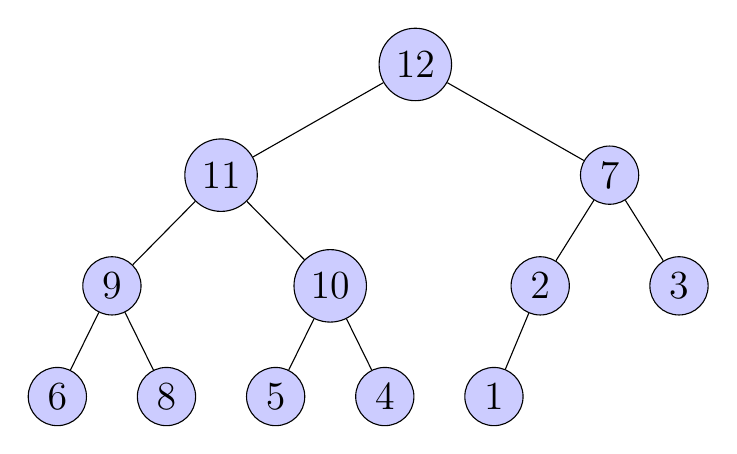
\begin{tikzpicture} [level distance = 40pt, sibling distance = 18pt,
  edge from parent/.style= { % added code
      draw, edge from parent path = {(\tikzparentnode) -- (\tikzchildnode)}}]
  \tikzset{every tree node/.style = 
    {align = center, circle, draw, fill = blue!20, font = \Large}}
    \Tree [.$12$
	    [.$11$
	       [.$9$ 
		$6$
		$8$
	       ]
	       [.$10$
		$5$
		$4$
	       ]
            ]
	    [.$7$ 
	      [.$2$
		$1$
		\edge[draw = none]; \node[draw = none, fill = none]{};
	      ]
	      $3$
	   ] 
        ]
\end{tikzpicture}
\end{document}

